The diagram (Figure 1) below shows the basic architectural layer diagram of the Beverage Management app. The overall structure of our app can be described using the popular three-layer architecture which consists of presentation layer, application layer and data access layer. The presentation layer is the top-most layer of our system which allows user to interact with the system. Application layer acts as an interface between the presentation layer and data access layer. This layer supports all of the core functions of our application. The data access layer is the layer where all the data and information are stored or retrieved from the database. In other words, the presentation layer takes input from the user and pass it to the application layer. The application layer then process those commands and pass the information to the data access layer. The data access layer either store the information on the database or retrieve the requested information from the database and pass it back to the application layer, and eventually to the presentation layer where the result is displayed in a user understandable format. 

\begin{figure}[h!]
	\centering
 	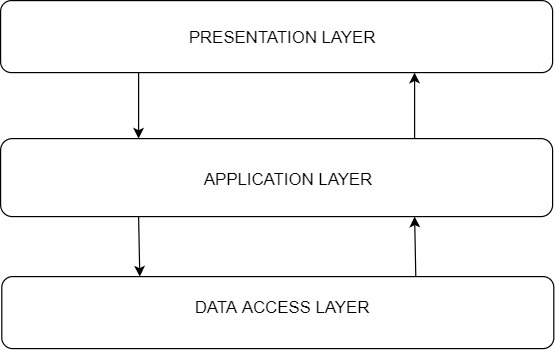
\includegraphics[width=0.60\textwidth]{images/ADS}
 \caption{A simple architectural layer diagram}
\end{figure}

\subsection{Presentation Layer Description}
This layer will allow our application to successfully communicate with the user. The features will include the display of login page, page for storing new products in the inventory, and also displaying the desired output for the user. This user level layer is connected with our application layer which will help to display or retrieve the required information that our user is looking for.

\subsection{Application Layer Description}
This layer will serve as a bridge between the presentation layer and data access layer of our application.  No matter what command the user gives in the presentation layer level, these commands will be interpreted by the application layer. Depending on the type of command, this layer will execute the command by accessing the database layer and then channels the accurate and expected output to the presentation layer.

\subsection{Database Access Layer Description}
This layer is the most fragile yet the most critical aspect of our application. This is where the information from the user is stored so that it can be accessed when required in future. We will be using subsytem such as Firebase, SQLite and Global barcode inventory. This layer will be the fulcrum to our team creating and effective management system. Multiple information will be recorded in this layer. This includes login credentials, a product’s name, flavor, type and so on. In brief, this layer will execute the query given by the user in presentation layer and process the result back to application layer which will finally process the information to be displayed in the presentation layer.